%
The frequency multiplexing of \NIKA\ prevents us from knowing {\it a priori} the pointing
direction of each detector on the sky. This has to be determined on
astronomical observations. We therefore scan a strong astromical source with the
entire focal plane. The calibration source, typically a planet (Mars, Uranus,
Neptune), is small compared to our beam and can be considered as a point
source. Indeed, during the 2012 observing campaign, the angular
diameter of Uranus was 3.54~arcsec. The convolution of the corresponding disk with a Gaussian beam of
13.5 and 18.4~arcsec FWHM would broaden our beam by only 0.17~arcsec at 1.25~mm and 0.12 at 2.14~mm.

The source is raster-scanned at 35~arcsec/s, and each subscan is 420~arcsec
long, centered on the source as the latter is being tracked by 
the telescope. This scanning speed provides about 10 and 12 points per FWHM at
  1.25~mm and 2.14~mm resp., hence providing excellent beam sampling. To
have a clean determination of the beam parameters (position, width, and
orientation) of each KID, we proceed in two steps.
 
\begin{enumerate} 
\item We apply a median filter of approximately 5~FWHM of width to the detector timelines to
  subtract most of the atmospheric signal and the low-frequency, correlated
  electronic noise while preserving most of the planet signal (less than 1~\% lost at scales 
  smaller than 2.5 x FWHM). These timelines
  are then projected onto individual maps per detector, and a Gaussian ellipse is
  fitted on the source. Centroid position provides a first estimate of the pointing
  parameters of each pixel. The amplitude of the Gaussian gives a calibration in
  Jy/Hz, where Hz represents the shift in resonant frequency 
  for each detector. If the atmospheric absorption is known and accounted for, this
  becomes a determination of the absolute calibration of each detector. If not,
  this can still be considered as a cross-calibration of KIDs all at once, and
  they can be combined accordingly into a single map of the source. This map
  provides the position of the source in sky coordinates.
\item With this information in hand, we can flag out the source in all KID
  timelines and build a template of the low frequency part of the signal (mostly
  sky noise and electronics noise) using, at each time, all detectors that are
  far from the source (typically further than a few beam FWHM,
  e.g.~30~arcsec). This template is then subtracted from each KID timeline. This
  leads to a clean determination of the planet signal with no filtering. Timelines
  are then projected a second time onto individual maps per KID, and a Gaussian
  elliptical fit provides the final pointing parameters and FWHM estimates.
\end{enumerate}

\begin{figure}[t!]
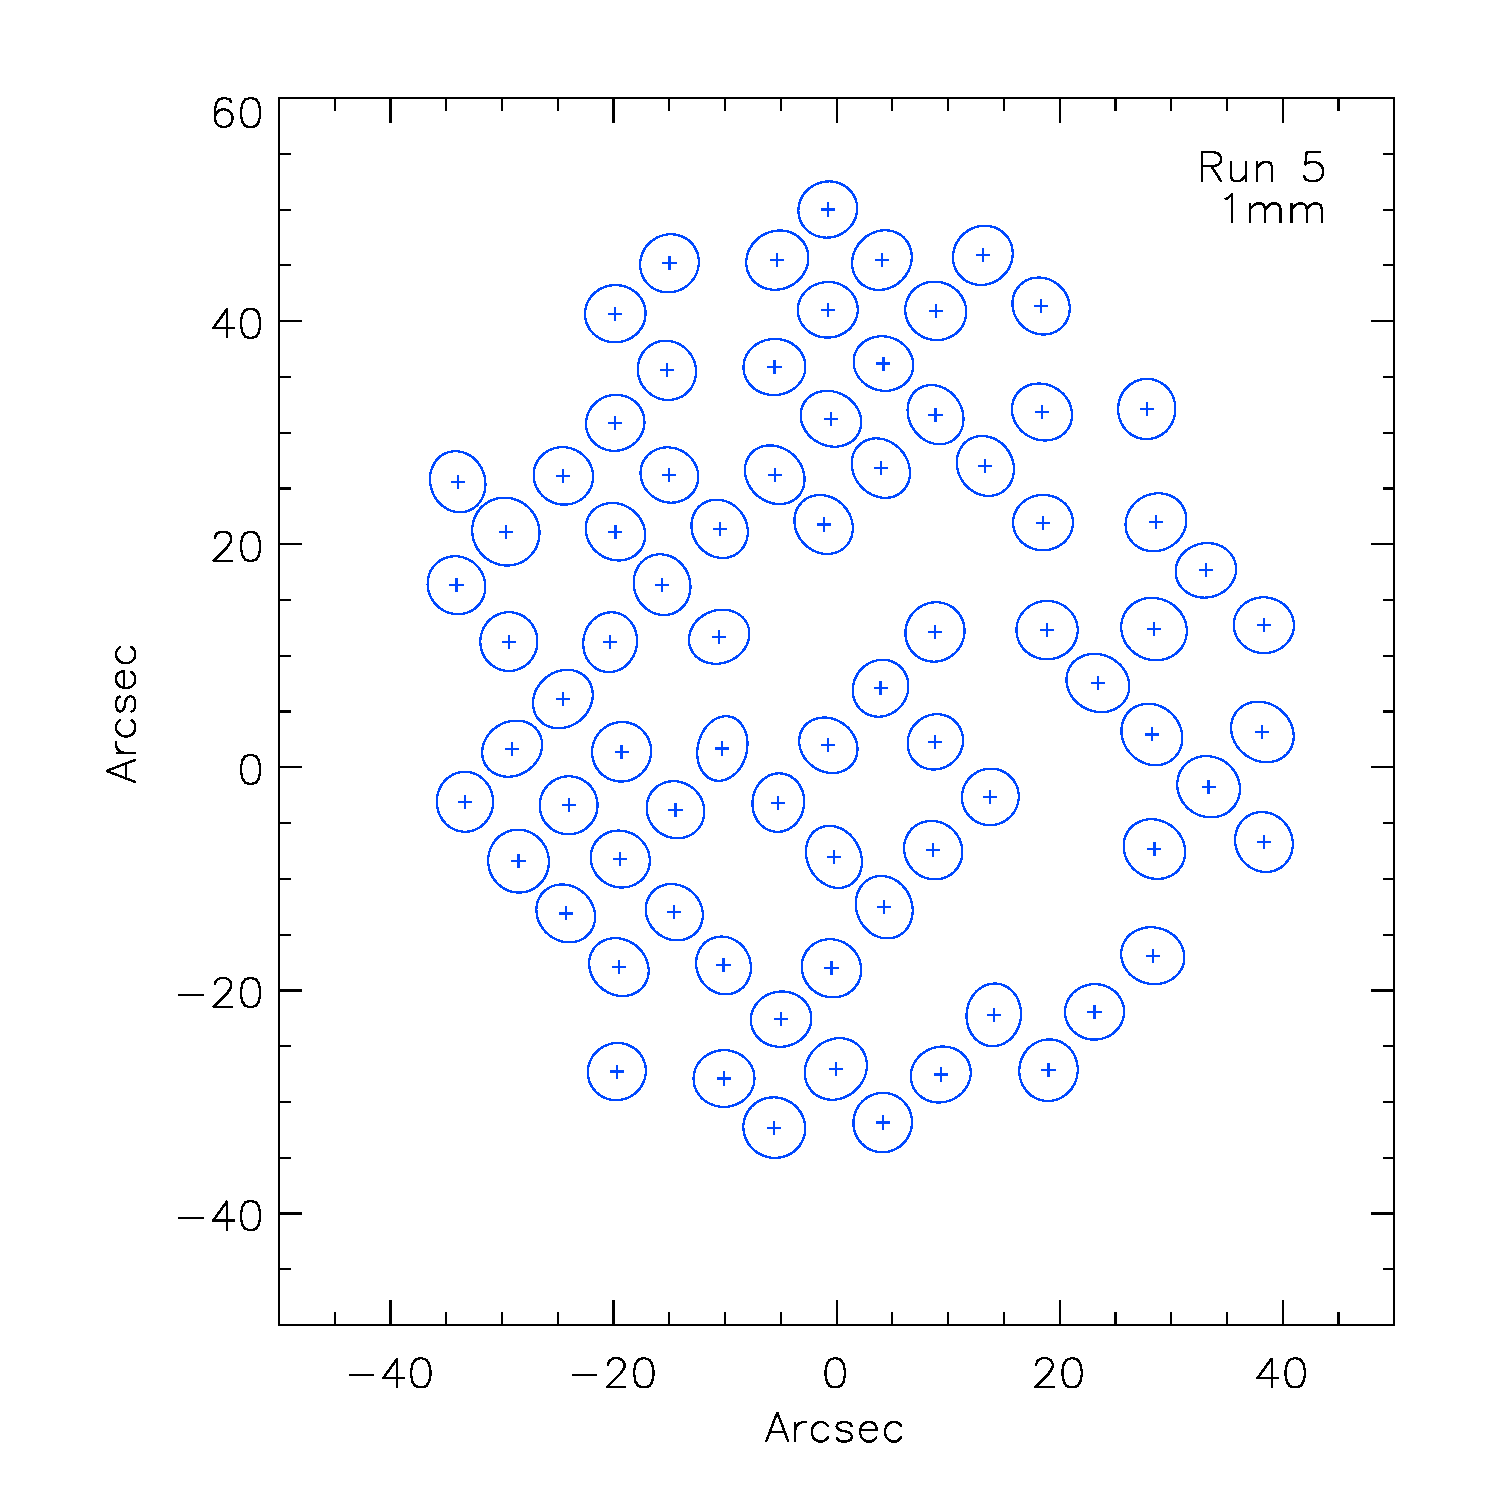
\includegraphics[width=4cm]{figures/run5_fpg_1mm.eps}
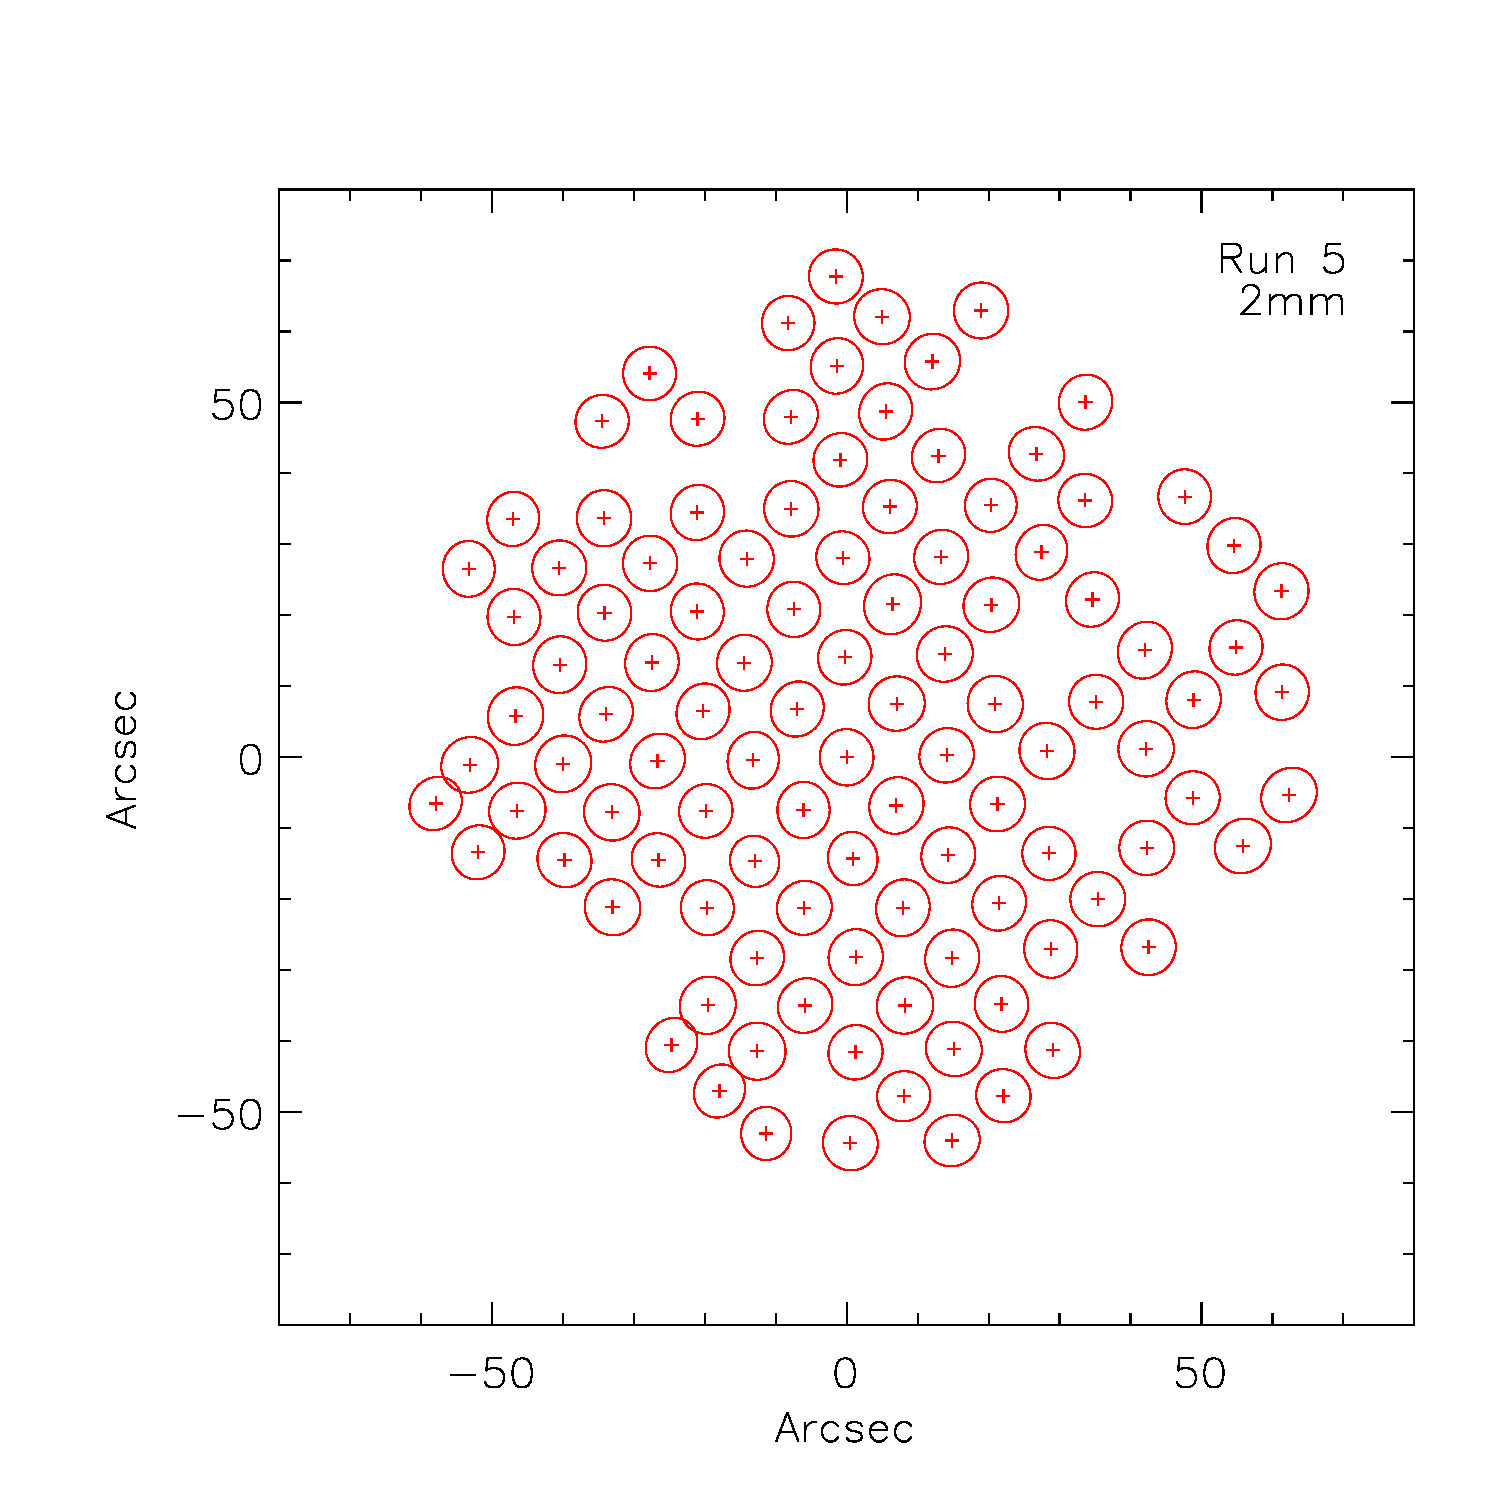
\includegraphics[width=4.2cm]{figures/run5_fpg_2mm.eps}\\
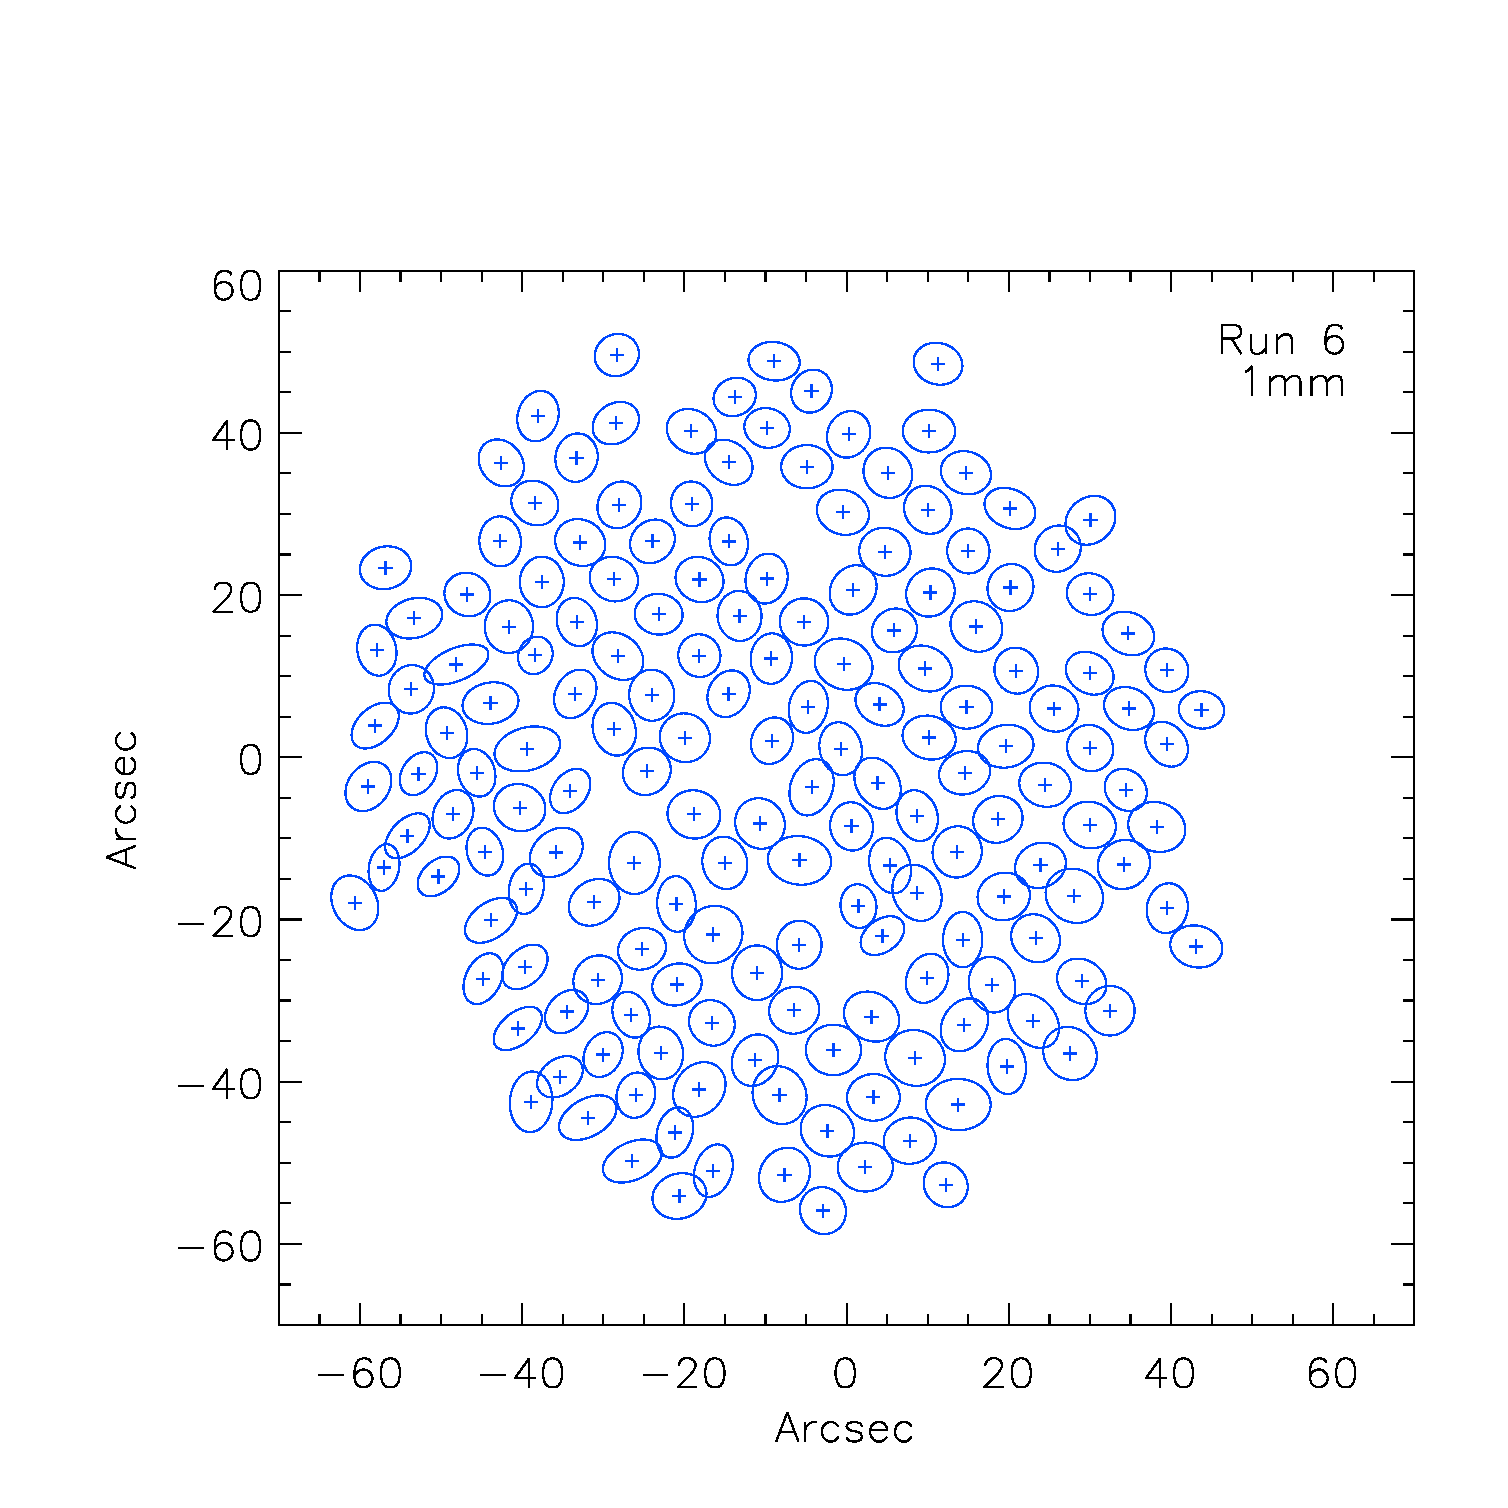
\includegraphics[width=4.3cm]{figures/run6_fpg_1mm.eps}
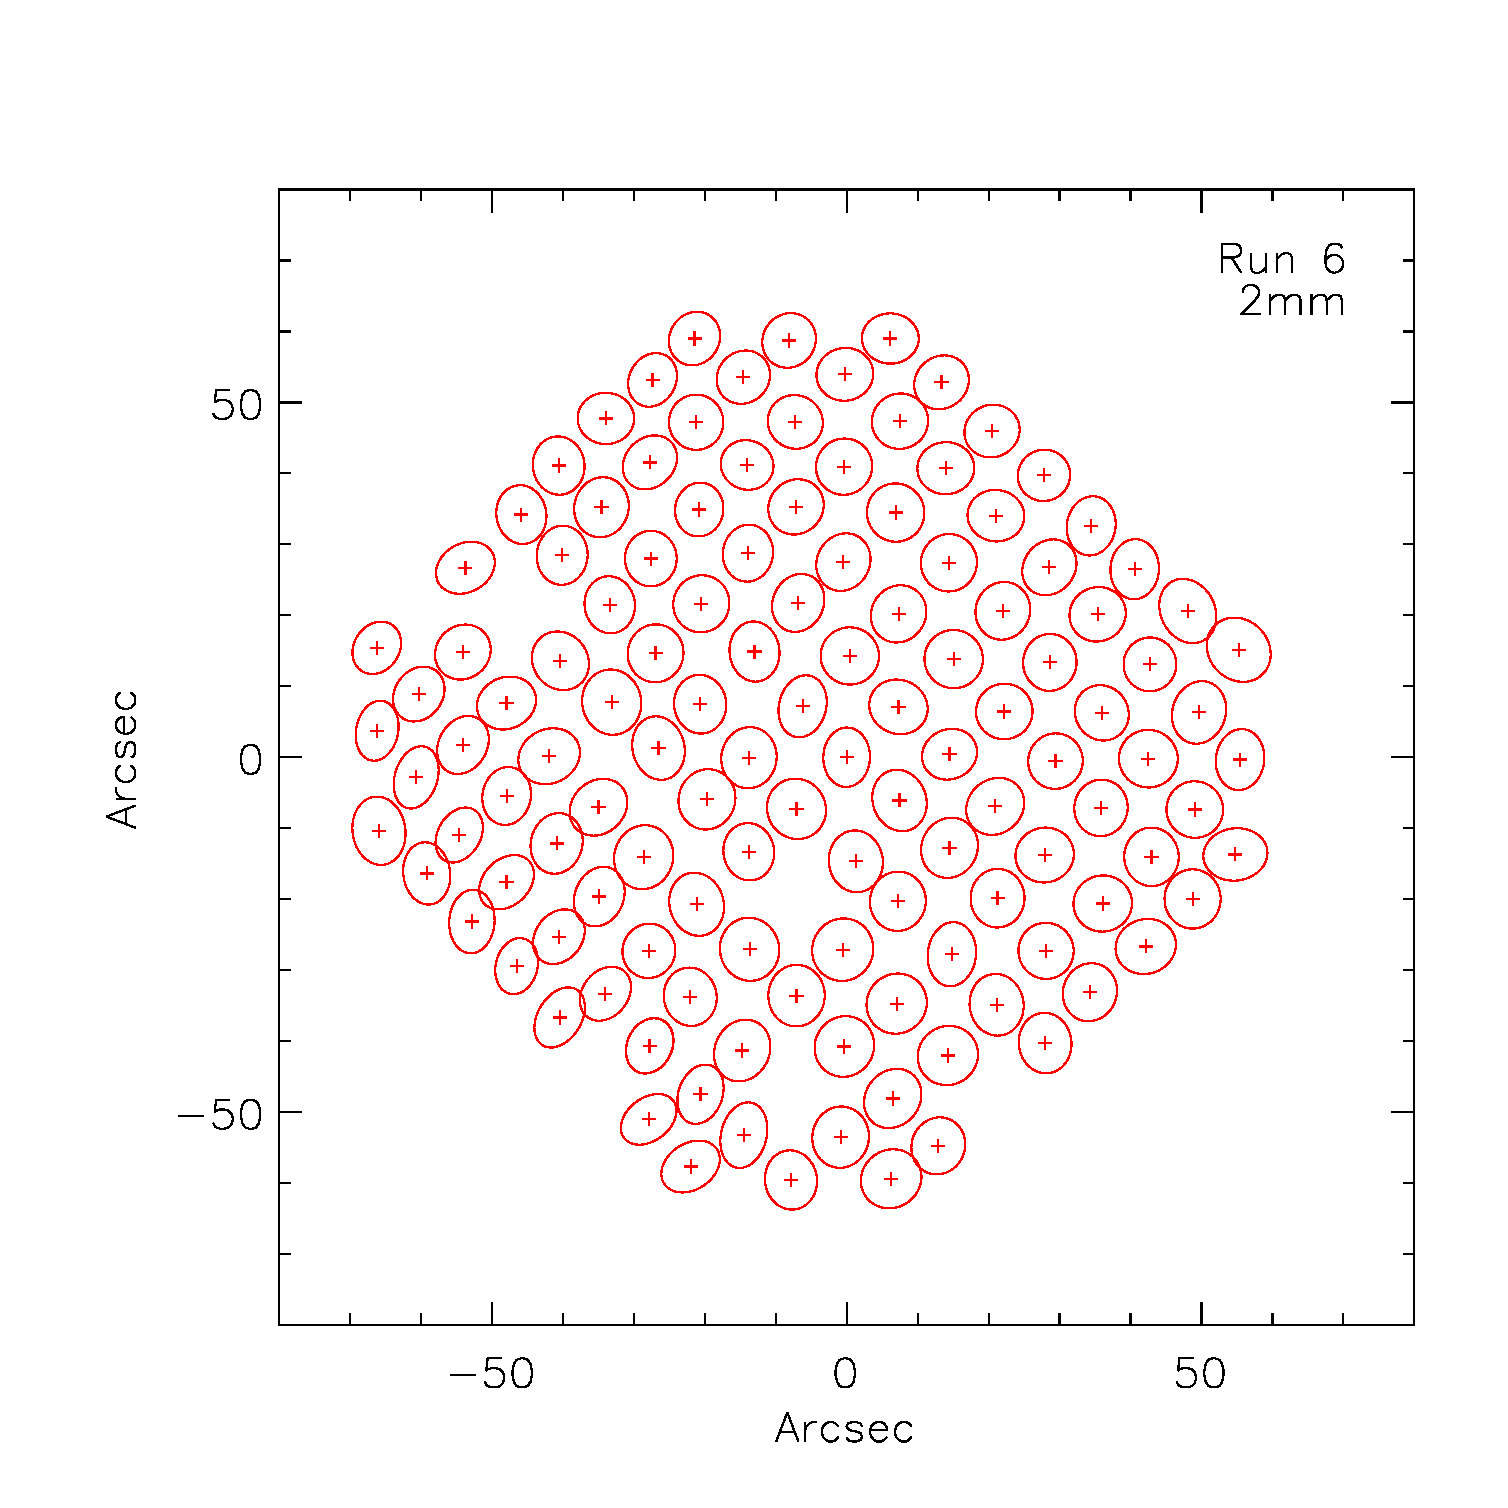
\includegraphics[width=4.1cm]{figures/run6_fpg_2mm.eps}
\caption{Detector sampling of the FOV at 1.25 mm (left) and 2.14 mm (right) for the 2012 (top) and 2013 (bottom) observing campaigns. Beam
  pattern contours have a diameter of $1\sigma=FWHM/\sqrt{8\ln 2}$.}
\label{fig:run6_fpg}
\end{figure}


\begin{figure}[t!]
\includegraphics[width=4.2cm]{figures/run5_beam_stats.eps}
\includegraphics[width=4.3cm]{figures/run6_beam_stats.eps}
\caption{Beam FWHM distribution at 1.25 (blue) and 2.14 (red)~mm for the 2012 (left) and 2013 (right) observing campaigns. 
The distribution of FWHMs was of lower quality during the 2013 observing campaign owing to
  poor weather conditions.}
\label{fig:run6_beam_stats}
\end{figure}

For illustration, Figures~\ref{fig:run6_fpg} and \ref{fig:run6_beam_stats} show
maps of the 1.25~mm and 2.14~mm detector images and the distribution of the
determined beam widths for the 2012 and 2013 observing campaigns. Several scans on
calibration sources are performed during the campaign to improve on the
reconstruction of the pointing. For the 2012 observing campaign, with typically
six such scans, we observed a median variation of the detector pointing
directions of 3.4~arcsec at 1.25~mm and 3.2 at 2.14~mm.
% for the 2013 observation campaign, even under poor weather
% conditions with opacities ranging from 0.5 to 0.9. 
Although beams were observed to be
a bit larger and asymmetric during 2013 observing campaign because of the weather conditions\footnote{Under turbulent sky, the anomalous refraction is larger and spreads the incoming light, hence enlarging the image.}, the number of valid pixels increased and the FOV was almost fully sampled. For the
2012 observing campaign, the average FWHM were $12.3\pm 0.2$~arcsec at 1.25~mm and $18.1 \pm 0.3$~arcsec
at 2.14~mm. For the 2013 observing campaign, they were $13.5\pm 0.9$ at 1.25~mm and
$18.4\pm0.8$~arcsec at 2.14~mm.
The combined beam is larger than individual detector beams because of a possible small offset in the reconstructed detector position in the FOV. 